
\input{slides_common.tex}

\tikzstyle{arrow} = [thick,->,>=stealth]
\tikzstyle{line} = [thick]

\tikzstyle{basic} = [rectangle, minimum height=1cm, text centered, draw=black, fill=white, text=black]
\tikzstyle{redstyle} = [draw=redBoxFg, fill=redBoxBg, text=redBoxFg]
\tikzstyle{yellowstyle} = [draw=yellowBoxFg, fill=yellowBoxBg, text=yellowBoxFg]
\tikzstyle{greenstyle} = [draw=greenBoxFg, fill=greenBoxBg, text=greenBoxFg]
\tikzstyle{bluestyle} = [draw=blueBoxFg, fill=blueBoxBg, text=blueBoxFg]
\tikzstyle{violetstyle} = [draw=violetBoxFg, fill=violetBoxBg, text=violetBoxFg]
\tikzstyle{nRedstyle} = [draw=nRedBoxFg, fill=nRedBoxBg, text=nRedBoxFg]
\tikzstyle{nGoldstyle} = [draw=nGoldBoxFg, fill=nGoldBoxBg, text=nGoldBoxFg]
\tikzstyle{nGreenstyle} = [draw=nGreenBoxFg, fill=nGreenBoxBg, text=nGreenBoxFg]
\tikzstyle{nBluestyle} = [draw=nBlueBoxFg, fill=nBlueBoxBg, text=nBlueBoxFg]
\tikzstyle{nPurplestyle} = [draw=nPurpleBoxFg, fill=nPurpleBoxBg, text=nPurpleBoxFg]
\tikzstyle{cheesyvertex} = [text width=2mm, text height=2mm, anchor=center]

\begin{document}

\hfill\myBiggerTitle{Exo-next (Spork of the Future)}

\vfill

\begin{centering}

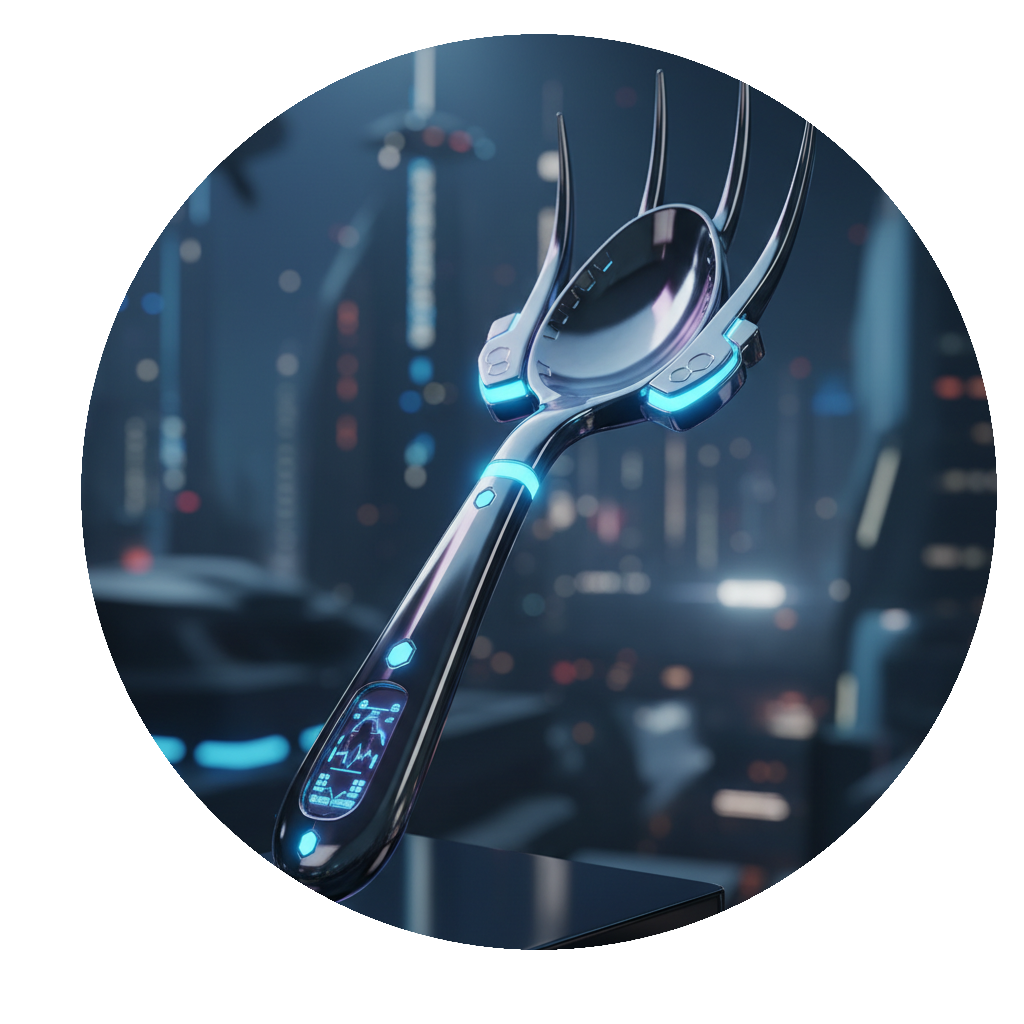
\includegraphics[width=0.5\linewidth]{spork_of_the_future.png}

\end{centering}

\vfill

\redBox{\LARGE For jrk's eyes only (for now)} \hfill Produced by Stupidly Still Using \textrm{\LaTeX} Studios

\newpage
\myBiggerTitle{OG Exo: The Good Stuff}

{\LARGE

Imperative mental model

\begin{itemize}
  \item Lower level control than pretty much any USL out there
  \item But we still know it's correct (if we use scheduling -- BIG IF)
  \item Not just memory hints or whatever
\end{itemize}

\vfill

Explicit instruction selection + valid usage checks (threads \& mem)

\begin{itemize}
  \item We \emph{genuinely} support user control over TMA and wgmma
  \item Maybe Blackwell
\end{itemize}

\vfill

Rewrite operations \myKeyA{as a convenience}

}

\newpage
\myBiggerTitle{Exo-GPU: The Good Stuff}

{\LARGE

Language-level parallelism

\begin{itemize}
  \item Express cooperation and programmer intent
\end{itemize}

\vfill

We reason about split barriers and async instrs -- not all PLs can

\vfill

``Unsafe by default'' abstract machine for synchronization checking

\begin{itemize}
  \item Write whatever you want, even if we can't statically analyze it
  \item Sound and complete(-ish), we give yes/no will-it-work for concrete sizes
  \item \myKeyA{If we implement Blackwell}, I'll have more confidence this is a reasonable ``bottom level'' abstraction.
\end{itemize}

\vfill

Orthogonal: ``dataflow/algorithm correct?'' and ``sync correct?''

}

\newpage
\myBiggerTitle{OG Exo: The Bad Stuff}

{\LARGE

It's \emph{too} ``literally'' imperative (\myKeyA{recurring theme}, to be elaborated)

\vfill

Terrible user experience for error messages
\begin{itemize}
  \item At least the ones \emph{\textrm{I}}, personally, did not write
  % \item But even then, for LLMs, structured error messages instead of plain text may be good
\end{itemize}

\vfill

Rewrite operations \myKeyA{as an obligation}
\begin{itemize}
  \item Only way to reason about correct dataflow/algorithm
\end{itemize}

\vfill

Scheduling myopia (also to be elaborated on)

\vfill

Control/data separation is a bummer
\begin{itemize}
  \item Affine indexing too
\end{itemize}

}

\newpage
\myBiggerTitle{Exo-GPU: The Bad Stuff}

{\LARGE

We are not CuTe (\myKeyA{recurring theme 2}, to be elaborated on)
\begin{itemize}
  \item Limited indexing abstraction, except for threads
  \item Number 1 emotional frustration with Exo codebase: deeply entrenched assumption that ``everything is a C pointer + strides''
\end{itemize}

\vfill

Constant integer restrictions cause grief
\begin{itemize}
  \item Slow parameter sweep, can't support variable \texttt{clusterDim}
  \item Inherited from Exo, but I made it way worse
\end{itemize}

\vfill

Implicit deductions for distributed memory and \texttt{cuda\_threads} loops
\begin{itemize}
  \item Hard to understand for everyone except David Zhao Akeley
  \item Good intentions: less cognitive load when scheduling
\end{itemize}

}

\newpage
\myBiggerTitle{Justification for Exo}

{\LARGE

Computers are imperative under the hood
\begin{itemize}
  \item Alloc buffers in explicit memory type
  \item Read \& write buffers in program order
  \item Free buffers
\end{itemize}

\vfill

$(\implies)$

Must expose true model (imperative) to optimize close-to-the-metal

\vfill

$(\implies)$

Invest in imperative IRs \& static analysis on imperative programs

\vfill

\hphantom{SPACER}

}

\newpage
\myBiggerTitle{Justification for Exo}

{\LARGE

Computers are imperative under the hood
\begin{itemize}
  \item Alloc buffers in explicit memory type
  \item Read \& write buffers in program order
  \item Free buffers
\end{itemize}

\vfill

\myKeyB{$(\implies)$ OK (Legion crowd may disagree, whatevs)}

Must expose true model (imperative) to optimize close-to-the-metal

\vfill

$(\implies)$

Invest in imperative IRs \& static analysis on imperative programs

\vfill

\hphantom{SPACER}

}

\newpage
\myBiggerTitle{Justification for Exo}

{\LARGE

Computers are imperative under the hood
\begin{itemize}
  \item Alloc buffers in explicit memory type
  \item Read \& write buffers in program order
  \item Free buffers
\end{itemize}

\vfill

\myKeyB{$(\implies)$ OK (Legion crowd may disagree, whatevs)}

Must expose true model (imperative) to optimize close-to-the-metal

\vfill

\myKeyA{$(\implies)$ This is suspect}

Invest in imperative IRs \& static analysis on imperative programs

\vfill

\hphantom{SPACER}

}

\newpage
\myBiggerTitle{Justification for Exo}

{\LARGE

``We want an imperative mental model for execution''

\begin{centering}

- and -

\end{centering}

``We want C-like programmer control''

\begin{centering}

\redBox{\emph{does not imply}}

\end{centering}

``Our object code has to be \emph{literally} like a subset of C''

}

\newpage
\myBiggerTitle{``Myopic'' Scheduling Operators}

{\LARGE

What does a scheduling operator do?

\begin{itemize}
  \item Look for where the cursor is pointing in IR tree
  \item Analyze relevant variables
  \item Traverse tree many times to find properties of variables
  \item Error if rewrite unsafe
  \item Construct modified tree
  \item Throw away everything we found out!!!
\end{itemize}

\vfill

Next scheduling operator starts with NO USEFUL INFORMATION

\vfill

We do this back-to-back hundreds or thousands of times

}

\newpage
\myBiggerTitle{My Intuition as a Programmer}

{\LARGE

What I have:

\myKeyA{Pure functional spec}

\begin{itemize}
    \item Histogram: bins $B(b)$, data $D(k)$, $B(b) = \sum_{k=0}^{K-1} \delta_{b, D(k)}$
    \item GEMM: $C(i, j) = \sum_{k=0}^{K-1} A(i, k) B(k, j)$
\end{itemize}

\myKeyA{Control Variables}

\myKeyB{Buffers}

\vfill

What I'm thinking: What do the \myKeyB{buffers} hold as a function of the \myKeyA{spec} and the \myKeyA{control variables}?
(What data @ what time?)

\vfill

In order to reason: do the output buffers hold the right values? \\
(This is somewhat like Allo, but I reason granularly, on all buffers)

}

\newpage
\myBiggerTitle{Histogram Intuition}

{\large
\input{nexo/histogram.0.tex}
}

{\LARGE

Functional spec: bins $B(b)$, data $D(k)$, $B(b) = \sum_{k=0}^{K-1} \delta_{b, D(k)}$
\begin{itemize}
    \item $\delta_{i,j}$ is the Kronecker delta, 1 if $i = j$ else 0
\end{itemize}

}

\newpage
\myBiggerTitle{Histogram Intuition}

{\large
\input{nexo/histogram.1.tex}
}

{\LARGE

Functional spec: bins $B(b)$, data $D(k)$, $B(b) = \sum_{k=0}^{K-1} \delta_{b, D(k)}$
\begin{itemize}
    \item $\delta_{i,j}$ is the Kronecker delta, 1 if $i = j$ else 0
\end{itemize}

\begin{equation*}
\texttt{tmp\_bins[$i$]} =
\begin{cases}
    0 & i \le \texttt{b} \\
    \textit{uninitialized} & i > \texttt{b}
\end{cases}
\end{equation*}

}

\newpage
\myBiggerTitle{Histogram Intuition}

{\large
\input{nexo/histogram.2.tex}
}

{\LARGE

Functional spec: bins $B(b)$, data $D(k)$, $B(b) = \sum_{k=0}^{K-1} \delta_{b, D(k)}$
\begin{itemize}
    \item $\delta_{i,j}$ is the Kronecker delta, 1 if $i = j$ else 0
\end{itemize}

\begin{align*}
\texttt{tmp\_bins[$b$]} &= \sum_{k'=0}^{\texttt{k}} \delta_{b, D(k')}
\end{align*}

(Partial histogram for first \texttt{k}-many data values)

}

\newpage
\myBiggerTitle{Histogram Intuition}

{\large
\input{nexo/histogram.3.tex}
}

{\LARGE

Functional spec: bins $B(b)$, data $D(k)$, $B(b) = \sum_{k=0}^{K-1} \delta_{b, D(k)}$
\begin{itemize}
    \item $\delta_{i,j}$ is the Kronecker delta, 1 if $i = j$ else 0
\end{itemize}

\begin{align*}
\texttt{tmp\_bins[$b$]} = \sum_{k'=0}^{K-1} \delta_{b, D(k')}
\end{align*}

}

\newpage
\myBiggerTitle{GEMM Intuition}

{\large
\input{nexo/gemm.0.tex}
}

{\LARGE

Functional spec: $C(i, j) = \sum_{k=0}^{K-1} A(i, k) B(k, j)$

}

\newpage
\myBiggerTitle{GEMM Intuition}

{\large
\input{nexo/gemm.1.tex}
}

{\LARGE

\vspace{-10mm}
\begin{gather*}
\texttt{A\_tile[$m,k$]} = \\
\begin{cases}
    A(m + (\greenBox{\texttt{m1}})(\texttt{M\_tile}), k + (\blueBox{\texttt{k1}})(\texttt{K\_tile}))
    &
    m < \greenBox{\texttt{m0}} \lor (m = \greenBox{\texttt{m0}} \land k \le \blueBox{\texttt{k0}}) \\
    \textit{uninitialized} & \text{otherwise}
\end{cases}
\end{gather*}

}

\newpage
\myBiggerTitle{GEMM Intuition}

{\large
\input{nexo/gemm.2.tex}
}

{\LARGE

\vspace{-10mm}
\begin{gather*}
\texttt{B\_tile[$k,n$]} = \\
\begin{cases}
    B(k + (\blueBox{\texttt{k1}})(\texttt{K\_tile}), n + (\violetBox{\texttt{n1}})(\texttt{N\_tile}))
    &
    k < \blueBox{\texttt{k0}} \lor (k = \blueBox{\texttt{k0}} \land n \le \violetBox{\texttt{n0}}) \\
    \textit{uninitialized} & \text{otherwise}
\end{cases}
\end{gather*}

}

\newpage
\myBiggerTitle{GEMM Intuition}

{\large
\input{nexo/gemm.3.tex}
}

{\LARGE

My intermediate reasoning on \texttt{A\_tile} and \texttt{B\_tile} informs my beliefs of the contents of \yellowBox{\texttt{C\_tile}}

}

\end{document}
